\InputIfFileExists{../data/global.src}\relax\relax

\iffull
\title[Erstes Tutorium -- Übungsblatt 1]{I've built this. With my \textit{bare} hands!}
\subtitle{Tutorium Eins}
\date{KW 18}
\addbibresource{references.bib}
\fi
\SetTutoriumNumber{1}

\iffull\begin{document}
\titleframe

\TopicOverview{1}
\fi


\SetNextSectionText{Practice yourself, for heaven's sake in little things, and then proceed to greater.\\--- Epictetus~\cite[adapted, chp.~16]{epictetusdiscourses}}
\setbox\pinguA=\hbox{\tikz{\pingu[right wing wave, laptop right,laptop right mid={\color{gray}\faLightbulbO},eyes wink,tie,glasses round,left wing grab]}}
\section{Präsenzaufgabe}
\begin{frame}[fragile]{Präsenzaufgabe}
\begin{aufgabe}{It's true, isn't it?}
\columns[c,onlytextwidth]
\column{.65\linewidth}
\begin{uncoverenv}<2->
\lstfs{10}\begin{plainjava}[aboveskip=-.65\baselineskip,belowskip=0pt]
class BoolescheAusdruecke {
   public static void main(String[] args) {

   }
}
\end{plainjava}
\end{uncoverenv}
\column{.35\linewidth}
    \onslide<3->{Erweitern Sie die Datei. Deklarieren und initialisieren sie benötigte Variablen mit \say{beliebigen} Werten.}
    \medskip
\endcolumns
\onslide<4->{Konstruieren Sie boolesche Ausdrücke, die folgendes abprüfen:\vspace*{-.5\topsep}}
\begin{itemize}
    \item<5-> Die Zimmertemperatur (\T{temperatur}) beträgt höchstens \num{22.5} Grad Celsius.
    \item<6-> Eine Person (\T{alter}) ist nicht zwischen 13 und 18 Jahre alt.\vspace*{-.75\topsep}
\end{itemize}
\onslide<7->{Geben Sie die Ergebnisse über \bjava{System.out.println(:lan:...:ran:)} aus.}
    \onslide<1->
\end{aufgabe}
\begin{tikzpicture}[overlay,remember picture]
    \onslide<8->{\node[above left,yshift=-2.525mm,xshift=2mm,scale=.95] at(current page.south east) {\copy\pinguA};}
\end{tikzpicture}
\end{frame}


\MakeThePinguExplainIt[text width=5.5cm,yshift=-5mm]{cap=!hide,vr-headset,vr-headset hair,body type=legacy,cup=!hide,lollipop left,right item angle=27}{Einen generell korrekten Datentyp gibt es selten. Diverse Bedingungen hängen vom Kontext ab.\medskip\\Die Zahlen sind erstmal beliebig.}
\begin{frame}[fragile,c]{Die Datentypen finden}
\DoAnimations
\begin{center}
    \task<2->{Zimmertemperatur höchstens \num{22.5} Grad Celsius, Alter nicht zwischen 13 und 18 Jahren.}
\end{center}
\begin{plainjava}
$2->$class BoolescheAusdruecke {
$2->$    public static void main(String[] args) {
$2->$        $8->$float $3->$temperatur = $9->$18.0f$3->$;
$2->$        $15->$short $10->$alter = $16->$15$10->$;
$18->$        // ...
$2->$    }
$2->$}$1->$
\end{plainjava}
\begin{tikzpicture}[overlay,remember picture,every path/.append style={line cap=round}]
    \onslide<4->{\node[above left,xshift=-1.75cm,yshift=1.65cm,yshift=\btdmfootheight] (t) at(current page.south east) {\strut Temperatur};}
    \onslide<5->{\node[below left=1mm,yshift=-1mm] (g) at (t.south) {\only<7->{\color{gray}}Ganzzahl}; \draw[thick,rounded corners=2pt] (t.south) -- ++(0,-.5mm) -| (g.north);}
    \onslide<6->{\node[below right=1mm,yshift=-1mm] (f) at (t.south) {Fließzahl}; \draw[thick,rounded corners=2pt] (t.south) -- ++(0,-.5mm) -| (f.north);}
    \onslide<7->{\node[below left=1mm,yshift=-1mm] (j1) at (f.south) {\solGet{keywordB}{float}};
        \node[below right=1mm,yshift=-1mm] (j2) at (f.south) {\only<8->{\color{gray}\ttfamily}\only<-7|handout:0>{\expandafter\solGet{keywordB}}{double}};
        \draw[thick,rounded corners=2pt] (f.south) -- ++(0,-.5mm) -| (j1.north);
        \draw[thick,rounded corners=2pt] (f.south) -- ++(0,-.5mm) -| (j2.north);
    }

    \onslide<11->{\node[above left,xshift=-6.1cm,yshift=1.56cm,yshift=\btdmfootheight] (t) at(current page.south east) {\strut Alter};}
    \onslide<12->{\node[below left=1mm,yshift=-1mm] (g) at (t.south) {Ganzzahl}; \draw[thick,rounded corners=2pt] (t.south) -- ++(0,-.5mm) -| (g.north);}
    \onslide<13->{\node[below right=1mm,yshift=-1mm] (f) at (t.south) {\only<14->{\color{gray}}Fließzahl}; \draw[thick,rounded corners=2pt] (t.south) -- ++(0,-.5mm) -| (f.north);}
    \onslide<14->{\node[below left=1mm,xshift=-1.15cm,yshift=-1mm] (j1) at (g.south) {\only<15->{\color{gray}\ttfamily}\only<-14|handout:0>{\expandafter\solGet{keywordB}}{byte}};
        \node[below left=1mm,xshift=2mm,yshift=-1mm] (j2) at (g.south) {\solGet{keywordB}{short}};
        \node[below right=1mm,yshift=-1mm] (j3) at (g.south) {\only<15->{\color{gray}\ttfamily}\only<-14|handout:0>{\expandafter\solGet{keywordB}}{int}};
        \node[below right=1mm,xshift=1.15cm,yshift=-1mm] (j4) at (g.south) {\only<15->{\color{gray}\ttfamily}\only<-14|handout:0>{\expandafter\solGet{keywordB}}{long}};
        \draw[thick,rounded corners=2pt] (g.south) -- ++(0,-.5mm) -| (j1.north);
        \draw[thick,rounded corners=2pt] (g.south) -- ++(0,-.5mm) -| (j2.north);
        \draw[thick,rounded corners=2pt] (g.south) -- ++(0,-.5mm) -| (j3.north);
        \draw[thick,rounded corners=2pt] (g.south) -- ++(0,-.5mm) -| (j4.north);
    }
    \onslide<0|handout:1>{\node[left=-4mm,xshift=5mm,scale=.8,yshift=\btdmfootheight] at(current page.-8) {\copy\pinguexplainbox};}% copy for animations
\end{tikzpicture}
\end{frame}

\begin{frame}[fragile,c]{Boolesche Ausdrücke konstruieren}
\DoAnimations
\begin{center}
    \task<2->{Zimmertemperatur \only<5|handout:0>{\textbf}{höchstens} \num{22.5} Grad Celsius, Alter \only<11|handout:0>{\textbf}{nicht} \only<10-11|handout:0>{\textbf}{zwischen 13 und 18 Jahren}.}
\end{center}
\SetupLstHl
% star uses only
% TODO: gray it out
\def\donumber{\solGet{numbers}}
\def\dokey{\solGet{keywordB}}
\def\dokeyC{\solGet{keywordC}}
\setbox0=\hbox{\solGet{basicsstyle}{\only<8-|handout:0>{\color{codeouthl}}temperatur~\onslide<5->{<=}~\only<-7>{\expandafter\donumber}{\slshape22.5}}}%
\setbox1=\hbox{\solGet{basicsstyle}{\onslide<11->{!(}\only<-11>{\expandafter\donumber}{\slshape13} \onslide<10->{<=} alter \onslide<10->{\&\&} alter \onslide<10->{<=} \only<-11>{\expandafter\donumber}{\slshape18}\onslide<11->{)}}}%
\begin{plainjava}
$2->$class BoolescheAusdruecke {
$2->$    public static void main(String[] args) {
$2->$        $2->{\text{\solGet{basicstyle}{\only<8-13|handout:0>{\color{codeouthl}}\only<-7,14->{\expandafter\dokey}{float} temperatur = \only<-7,14->{\expandafter\donumber}{\slshape18.0}f;}}}$
        $2->{\text{\solGet{basicstyle}{\only<3-7|handout:0>{\color{codeouthl}}\only<-2,8->{\expandafter\dokey}{short} alter = \only<-2,8->{\expandafter\donumber}{\slshape15};}}}$
        $6->{\text{\solGet{basicsstyle}{\only<8-13|handout:0>{\color{codeouthl}}\only<7->{{\only<-7,14->{\expandafter\dokeyC}{System}.out.println(}}\tikzmarknode{SE-EQUALS-MAY-RISE}{\solGet{basicsstyle}{\only<8-13|handout:0>{\color{codeouthl}}temperatur <= \only<-7,14->{\expandafter\donumber}{\slshape22.5}f}}\only<7->{);}}}}$
        $12->{\text{\solGet{basicsstyle}{\only<13->{{\dokeyC{System}.out.println(}}\tikzmarknode{BRAVE-NEW-WORLD}{\solGet{basicsstyle}{!(\donumber{13} <= alter \&\& alter <= \donumber{18})}}\only<13->{);}}}}$
$2->$    }
$2->$}$1->$
\end{plainjava}
\begin{tikzpicture}[overlay,remember picture,every path/.append style={line cap=round}]
    \onslide<4-11|handout:0>{\node[above left=.5cm+\btdmfootheight] (@) at(current page.south east) {\box0};}
    \onslide<9-13|handout:0>{\node[above left=.5cm+\btdmfootheight,xshift=-5cm] (@c) at(current page.south east) {\box1};}
    \onslide<6-11|handout:0>{
        \scope
        \only<8-|handout:0>{\color{codeouthl}}
        \draw[decoration={brace,amplitude=3pt},decorate] (SE-EQUALS-MAY-RISE.south east) to  coordinate[pos=.5,yshift=-2mm] (@b) (SE-EQUALS-MAY-RISE.south west);
    \draw[-Kite] (@.north) to[out=140,in=320] (@b);
    \endscope }
    \onslide<12-13|handout:0>{
        \draw[decoration={brace,amplitude=3pt},decorate] (BRAVE-NEW-WORLD.south east) to  coordinate[pos=.5,yshift=-2mm] (@d) (BRAVE-NEW-WORLD.south west);
        \only<12|handout:0>{
            \draw[-Kite] (@c.north) to[out=100,in=280] (@d);
        }
        \only<13->{
            \draw[-Kite] (@c.north) to[out=80,in=260] (@d);
        }
    }
    \only<15->{\node[above left,yshift=\btdmfootheight] at (current page.south east) {\textattachfile{BoolescheAusdruecke.java}{BoolescheAusdruecke.java}\;};}
\end{tikzpicture}\relax
\end{frame}
% 14. 4
\def\hlcode#1#2{\fill[paletteA,opacity=.2,rounded corners=1pt] ([shift={(-.5mm,2pt)}]#1.south west) rectangle ([shift={(.5mm,-2pt)}]#1.north east); \coordinate (#2) at (#1.east);}
\begin{frame}[fragile]{Deklarieren, Initialisieren und Zuweisen}
    \begin{itemize}
        \itemsep10pt
        \item<2-> Die Begriffe sind leicht definiert:
        \begin{description}[Initialisierung:]
            \itemsep2pt
            \item<3->[Deklaration:] Reserviert einen Namen und setzt den Typ\hfill \onslide<4->{\bjava{int x, y;}}
            \item<7->[Initialisierung:] Die \textit{erste} Zuweisung einer Variable\hfill\onslide<8->{\info{Erst jetzt ist die Variable verwendbar}}
            \item<5->[Zuweisung:] Setzen/Ändern des Wertes einer Variable\hfill\onslide<6->{\bjava{x = 3;}}
        \end{description}
    \end{itemize}\vspace*{6mm}
\lstfs{10}
\begin{plainjava}[lineskip=4.35pt]
!*\onslide<10->*!public static void main(String[] args) {
    !*\tikzmarknode{temperatur}{\solGet{basicstyle}{\solGet{keywordB}{int} \strut apfelsine}}*!;
    !*\tikzmarknode{alter}{\solGet{basicstyle}{\solGet{keywordB}{char} \strut zeichen = \solGet{literals}{'x'}}}*!;
    !*\tikzmarknode{temperatur2}{\solGet{basicstyle}{\strut apfelsine = \solGet{numbers}{42}}}*!;
    if(apfelsine % 2 == 0)    !*\tikzmarknode{rightmark}{}*!
        !*\tikzmarknode{alter2}{\solGet{basicstyle}{\strut zeichen = \solGet{literals}{'k'}}}*!;
}
\end{plainjava}
\begin{tikzpicture}[overlay,remember picture,T/.style={sol@colors@lst@comments,font=\itshape\sffamily\footnotesize}]
    \onslide<11->{\hlcode{temperatur}{@a}} \onslide<12->{\node[right=3mm,T] at(@a-|rightmark.east) {\textbf{Deklarierung} einer Variable \say{apfelsine} vom Typ \T{int}};}
    \onslide<11->{\hlcode{alter}{@c}} \onslide<13->{\node[right=3mm,T] at(@c-|rightmark.east) {\textbf{Deklarierung} mit Typ \T{char} und \textbf{Initialisierung} mit dem Wert \T{'x'}};}
    \onslide<11->{\hlcode{temperatur2}{@b}} \onslide<14->{\node[right=3mm,T] at(@b-|rightmark.east) {\textbf{Initialisierung} mit dem Wert \T{42}};}
    \onslide<11->{\hlcode{alter2}{@d}} \onslide<15->{\node[right=3mm,T] at(@d-|rightmark.east) {\textbf{Zuweisung} des Wertes \T{'k'}};}
\end{tikzpicture}
        % TODO: beispiel an Programm TODO: OPerationen bei Rechnung mit eintragen TODO: aufwändigere Aufwandsanalyse ;) TODO: endlichkeit und halteproblem TODO: korrekt zitat von Knuth bei Verifikation  TODO: termiation: Länge ist fest
\end{frame}

\SetNextSectionText{Algorithmenentwurf und -analyse\\Abgabe: \DTMDate{2022-05-02}}
\section{Übungsblatt 1}
\subsection{Aufgabe 1}
{
\setbeamertemplate{enumerate item}{\task{\alph{enumi})}}
\begin{frame}[t]{Aufgabe 1: Aufwandsanalyse}
    \task<2->{\task{\onslide<2->{In der Vorlesung haben wir uns mit der Aufwandsanalyse von Algorithmen beschäftigt und uns angeschaut, wie viele
    Operationen im schlechtesten Fall notwendig sind, um den Algorithmus durchzuführen. Im Folgenden wollen wir uns
    nun anschauen, wie sich solche Aussagen (vereinfacht) auf Maschinenoperationen übetragen lassen.}

    \onslide<3->{Bei einer Firma fällt im Produktionsprozess täglich ein Optimierungsproblem an, für dessen Lösung eine Stunde zur
    Verfügung steht. Der Algorithmus zur Lösung des Optimierungsproblems muss bei Eingabe eines Problems der Größe \(n\) insgesamt \(100n^2\) viele Operationen durchführen.
    Bisher verwendet die Firma zur Lösung einen Mikro-Rechner mit einem Prozessortakt von \(\qty{800}{\mega\hertz}\). Dieser kann in
    jeder Sekunde \(\num{40000}\) der oben genannten Operationen berechnen.}
    \begin{enumerate}
            \item<4-> \task{Welche Problemgröße \(n\) dürfen die Probleme maximal haben, damit die Berechnung innerhalb der Frist
            durchgeführt werden kann?}
            \item<5-> \task{Nun soll auf einen schnelleren Rechner mit \(\qty{3200}{\mega\hertz}\) Taktfrequenz umgestiegen werden. Nehmen Sie an, die
            höhere Taktfrequenz übersetze sich direkt in eine entsprechend höhere Rechengeschwindigkeit. Wie groß können
            nun die Optimierungsprobleme sein?}
            \item<6-> \task{Anstelle einer CPU mit einem, soll eine CPU mit 16 Kernen (jeweils mit \(\qty{3200}{\mega\hertz}\)) eingesetzt werden.
            Glücklicherweise lässt sich das Optimierungsproblem leicht parallelisieren, so dass sich die Geschwindigkeit im
            Vergleich zu einem Kern verneunfacht. Wie groß können nun die Optimierungsprobleme sein?}
    \end{enumerate}}}
\end{frame}

\begin{frame}{Aufwandsobergrenze}
\only<handout:0>{\task<2->{Tägliches Optimierungsproblem für dessen Lösung eine Stunde zur
Verfügung steht. Der Algorithmus zur Lösung benötigt bei Eingabe eines Problems der Größe \(n\) insgesamt \(100n^2\) Operationen.
Der Mikro-Rechner mit einem Prozessortakt von \(\qty{800}{\mega\hertz}\) kann in
jeder Sekunde \(\num{40000}\) obiger Operationen berechnen.}}
\begin{enumerate}
    \item<3-> \task{Was ist die maximale Problemgröße \(n\) um in der Frist zu bleiben?\medskip}
    \onslide<4->{In der Stunde haben wir \(60 \cdot 60\) Sekunden und damit \(60 \cdot 60 \cdot \num{40000}\) Operationen. Bei Problemgröße \(n\) benötigen wir \(100n^2\) Operationen:} \shortmathskip\begin{align*}
        \onslide<5->{100n^2} &\onslide<5->{\leq 60 \cdot 60 \cdot \num{40000}}\\
        \onslide<6->{100n^2} &\onslide<6->{\leq \num{144000000}} && \mid {}\cdot{} \sfrac1{100}\quad \mid \sqrt{\phantom{a:}}\\
        \onslide<7->{n}      &\onslide<7->{\leq \sqrt{\num{1440000}}}\\
        \onslide<8->{n}      &\onslide<8->{\leq 1200}
     \end{align*}
     \onslide<9->{\faAngleRight~Die Problemgröße \(n\) darf \(1200\) nicht übersteigen.}
\end{enumerate}
\end{frame}

\begin{frame}{Die Macht der Taktfrequenz}
\only<handout:0>{\task<2->{Tägliches Optimierungsproblem für dessen Lösung eine Stunde zur
Verfügung steht. Der Algorithmus zur Lösung benötigt bei Eingabe eines Problems der Größe \(n\) insgesamt \(100n^2\) Operationen.
Der Mikro-Rechner mit einem Prozessortakt von \(\qty{800}{\mega\hertz}\) kann in
jeder Sekunde \(\num{40000}\) obiger Operationen berechnen.}}
\begin{enumerate}
    \setcounter{enumi}{1}
    \item<3-> \task{Angenommen, die
    höhere Taktfrequenz übersetze sich direkt in eine entsprechend höhere Rechengeschwindigkeit. Wie groß können
    die Optimierungsprobleme bei \(\qty{3200}{\mega\hertz}\) Taktfrequenz sein?\medskip}
    \onslide<4->{Bisher schaffen wir \(\num{40000}\) Operationen, nun schaffen wir \(\num{40000} \cdot \sfrac{\qty{3200}{\mega\hertz}}{\qty{800}{\mega\hertz}}\):}
    \shortmathskip\begin{align*}
        \onslide<5->{100n^2} &\onslide<5->{\leq 60 \cdot 60 \cdot \num{40000} \cdot \sfrac{\qty{3200}{\mega\hertz}}{\qty{800}{\mega\hertz}}}\\
        \onslide<6->{100n^2} &\onslide<6->{\leq \num{576000000}} && \mid {}\cdot{} \sfrac1{100}\quad \mid \sqrt{\phantom{a:}}\\
        \onslide<7->{n}      &\onslide<7->{\leq \sqrt{\num{5760000}}}\\
        \onslide<8->{n}      &\onslide<8->{\leq 2400}
     \end{align*}
     \onslide<9->{\faAngleRight~Die Problemgröße \(n\) darf nun \(2400\) nicht übersteigen.}
     \onslide<10->{\infoblock{Ein vervierfachen der Leistung verdoppelt die mögliche Problemgröße aufgrund des quadratischen Wachstums.}}
\end{enumerate}
\end{frame}

\begin{frame}{Parallelisierungskosten}
    \only<handout:0>{\task<2->{Tägliches Optimierungsproblem für dessen Lösung eine Stunde zur
    Verfügung steht. Der Algorithmus zur Lösung benötigt bei Eingabe eines Problems der Größe \(n\) insgesamt \(100n^2\) Operationen.
    Der Mikro-Rechner mit einem Prozessortakt von \(\qty{800}{\mega\hertz}\) kann in
    jeder Sekunde \(\num{40000}\) obiger Operationen berechnen.}}
    \begin{enumerate}
        \setcounter{enumi}{2}
        \item<3-> \task{Anstelle einer CPU mit einem, soll eine CPU mit 16 Kernen (jeweils mit \(\qty{3200}{\mega\hertz}\)) eingesetzt werden.
        Glücklicherweise lässt sich das Optimierungsproblem leicht parallelisieren, so dass sich die Geschwindigkeit im
        Vergleich zu einem Kern verneunfacht. Wie groß können nun die Optimierungsprobleme sein?\medskip}
        \onslide<4->{Die Anzahl der Operationen verneunfacht sich direkt:}
        \shortmathskip\begin{align*}
            \onslide<5->{100n^2} &\onslide<5->{\leq 60 \cdot 60 \cdot \num{40000} \cdot \sfrac{\qty{3200}{\mega\hertz}}{\qty{800}{\mega\hertz}}} \\
            \onslide<6->{100n^2} &\onslide<6->{\leq \num{5184000000}} && \mid {}\cdot{} \sfrac1{100}\quad \mid \sqrt{\phantom{a:}}\\
            \onslide<7->{n}      &\onslide<7->{\leq \sqrt{\num{51840000}}}\\
            \onslide<8->{n}      &\onslide<8->{\leq 7200}
            \end{align*}
            \onslide<9->{\faAngleRight~Die Problemgröße \(n\) darf nun \(7200\) nicht übersteigen.}
    \end{enumerate}
\end{frame}

\iffull
{\AddonFrame
\begin{frame}{Laufzeitabschätzungen}
    \begin{itemize}[<+(1)->]
        \itemsep17pt
        \item Wir bekommen in der Regel \info{leider} nichts geschenkt.
        \begin{itemize}
            \itemsep3.5pt
            \item Parallelisierung ist mit Kosten verbunden.
            \item Wir müssen die parallelen Abläufe koordinieren, abgleichen,~\ldots
            \item Je nach Optimierung und Problem kann mehr Parallelisierung sogar schädlich sein!
            \item Auch ist nie alles parallelisierbar (Initialisierungen, Ausgaben,~\ldots).\onslide<+(1)->{\infoblock{Eine pessimistische Abschätzung liefert das \say{Amdahlsche Gesetz}~(wer mag:~\cite{amdahl1967amdahl}).}}
        \end{itemize}
        \item Für die Skalierung hat \(n\)\raisebox{3pt}{\scriptsize2} einen viel größeren Einfluss, als der Faktor \(100\) \begin{itemize}
            \itemsep3.5pt
            \item So vervielfachen 16 CPUs mit je vierfacher Leistung die Performanz um lediglich \(6\)!
            \item Meist interessiert uns nur das Wachstumsverhalten (polynomiell, exponentiell,~\ldots)
        \end{itemize}
    \end{itemize}
\end{frame}}
\fi
}

\subsection{Aufgabe 2}
{\setbeamerfont{description item}{series=\sbseries}
\begin{frame}{Aufgabe 2: Korrektheit von Algorithmen}
\columns[onlytextwidth,c]
\column{.6\linewidth}
\task<2->{Betrachten Sie die Anweisungsfolge. Handelt es sich hierbei um einen Algorithmus? Prüfen Sie \emph{alle} notwendigen Voraussetzungen.}
\column{.4\linewidth}% fake the design :)
\task<3->{\begin{tabular}{r<{:}@{\hskip1ex}ll}
    1 & Setze & \(x = 1\) \\
    2 & \textbf{solange} & \(x \geq 0\) \textbf{wiederhole}\\
    3 & & Verdopple \(x\) \\
    4 & & Verringere \(x\) um \(1\) \\
    5 & \textbf{ende} & \\
\end{tabular}}
\endcolumns\bigskip
\begin{description}[Terminiert:]
    \itemsep6pt
    \item<4->[Ausführ- und Reproduzierbarkeit:] \strut\onslide<5->{Ja, alle Schritte sind klar und umsetzbar.}
    \item<6->[Von Prozessor schrittweise ausführbar:] \strut\onslide<7->{Ja, ein Mensch kann sie auf Papier durchführen.}
    \item<8->[Nur Elementaroperationen \info{oder in solche übersetzbar}:] \strut\onslide<9->{Ja, für alle per Definition.}
    \item<10->[Endliche Beschreibung:] \strut\onslide<11->{Ja, per der Beschreibungstext ist endlich.}
    \item<12->[Terminiert:] \strut\onslide<13->{Nein, es handelt sich um eine Endlosschleife. Die Werte von \T{x} verhalten sich \(1 \to 2 \to 1 \to 2 \to \ldots\), damit ist nie \(x \geq 0\).}
\end{description}
\end{frame}}
\iffull
{\AddonFrame
\begin{frame}{Die Sache mit dem Terminieren}
    TODO: Ausflug: Halteproblem
\end{frame}
}
\fi

\subsection{Aufgabe 3}
% compensate for fat overflow
\newcommand<>\hlkw[1]{{\savebox0{#1}\only#2{\bfseries\color{paletteA}}\makebox[\dimexpr\wd0+.285ex]{\strut#1}}}
\newcommand<>\hloutkw[1]{{\savebox0{#1}\only#2{\bfseries\color{paletteB}}\makebox[\dimexpr\wd0+.285ex]{\strut#1}}}
\def\g#1{{#1}}\def\k#1{{\savebox0{#1}\makebox[\dimexpr\wd0+.285ex]{\strut#1}}}
\def\gk#1{\g{\k{#1}}}
\newcommand<>\hgk[1]{\hloutkw#2{\g{\k{#1}}}}
\iffull
\begin{frame}[c]{Aufgabe 3: Algorithmenkonstruktion}
    \pause\centering \parbox{.7\linewidth}{%
    \footnotesize\color{gray}\footnotesize Angenommen, Sie überlegen sich ein \g{neues Tablet} für die \g{Uni} zu kaufen.
    Sie stellen jedoch fest, dass die \g{Preise für elektronische Geräte} durch den \g{Chipmangel} in \g{letzter Zeit} stark gestiegen sind.
    Nun haben Sie eine \g{Website} gefunden, die Ihnen die jeweiligen \g{\k{Tagespreise}} eines Tablets über die \g{letzten Monate} liefert.
    Sie möchten nun den \g{\k{maximalen prozentualen Preisanstieg}} zwischen \g{\k{zwei aufeinanderfolgenden Tagen}} für dieses Tablet herausfinden.\bigskip\par
    Entwickeln Sie einen \g{Algorithmus}, der aus einer \hgk<4->{Liste} \hgk<4->{von} \hgk<4->{Tagespreisen} des Tablets den \hloutkw<4->{maximalen prozentualen Preisanstieg} von \hgk<4->{zwei} \hgk<4->{aufeinan\rlap{-}}\allowbreak\hgk<4->{derfolgenden} \hgk<4->{Tagen} berechnet.}\only<5->{\qquad\parbox{.2\linewidth}{%
        \centering\footnotesize \onslide<6->{\paletteA{Liste von Tagespreise}\\{\color{gray}\((p_1,\;\ldots,\;p_n)_{n\in\N}\)}\medskip\par
        \onslide<7->{\faCaretDown\medskip\par \paletteB{Max. \% Preisanstieg}\\{\color{gray}\(\DeltaMax\)}}}
    }}
\end{frame}

{\def\g#1{{\only<2->{\color{black}}#1}}\def\k#1{{\savebox0{#1}\only<3->{\bfseries\color{paletteA}}\makebox[\dimexpr\wd0+.285ex]{\strut#1}}}
\renewcommand<>\hlkw[1]{{\savebox0{#1}\makebox[\dimexpr\wd0+.285ex]{\strut#1}}}
\renewcommand<>\hloutkw[1]{{\savebox0{#1}\makebox[\dimexpr\wd0+.285ex]{\strut#1}}}
\def\gk#1{\g{\k{#1}}}
\begin{frame}[c]{Aufgabe 3}
    \centering \parbox{.7\linewidth}{\color{gray}\footnotesize Angenommen, Sie überlegen sich ein \g{neues Tablet} für die \g{Uni} zu kaufen.
    Sie stellen jedoch fest, dass die \g{Preise für elektronische Geräte} durch den \g{Chipmangel} in \g{letzter Zeit} stark gestiegen sind.
    Nun haben Sie eine \g{Website} gefunden, die Ihnen die jeweiligen \g{\k{Tagespreise}} eines Tablets über die \g{letzten Monate} liefert.
    Sie möchten nun den \g{\k{maximalen prozentualen Preisanstieg}} zwischen \g{\k{zwei aufeinanderfolgenden Tagen}} für dieses Tablet herausfinden.\bigskip\par
    Entwickeln Sie einen \g{Algorithmus}, der aus einer \hgk<4->{Liste} \hgk<4->{von} \hgk<4->{Tagespreisen} des Tablets den \hloutkw<4->{maximalen prozentualen Preisanstieg} von \hgk<4->{zwei} \hgk<4->{aufeinan\rlap{-}}\allowbreak\hgk<4->{derfolgenden} \hgk<4->{Tagen} berechnet.}\qquad\parbox{.2\linewidth} Preisanstieg}\smallskip\\
    }
\end{frame}
}
\fi
{\setbeamerfont{description item}{series=\sbseries}
\begin{frame}{Problemspezifikation}
\begin{description}[Tag]
    \itemsep9pt
    \item<+(1)->[Tagespreis:] positive reelle Zahl. Dargestellt mit zwei Nachkommastellen.
    \item<+(1)->[Tagespreisliste:] chronologisch sortierte Liste an Tagespreisen \([p_1, \ldots, p_n]\) mit \(n \in \N_1\).
    \item<+(1)->[Tag:] natürlicher Index in Tagespreisliste.
    \item<+(1)->[Zwei aufeinanderfolgende Tage:] zwei Listenindizes: \(i\) und \(i + 1\) \info{wobei \(i, i + 1 < n\)}.
    \item<+(1)->[Preisanstieg:] positive Veränderung einer reellen Zahl (dem Tagespreis): \(p_{i + 1} - p_i > 0\).
    \item<+(1)->[Maximaler prozentualer Preisanstieg:] größter relativer Preisanstieg: \(\max_{1 \leq i < n} \frac{p_{i + 1} - p_i}{p_i} \cdot 100\).\medskip
\end{description}
\onslide<+(1)->{\infoblock{\textbf{Wichtig:} Wir sind hier nicht in einer Programmiersprache: Typen wie \say{\bjava{int}} gibt es nicht $\implies$ mathematische Notation benutzen oder eigenen Typ definieren (wie Tupel, \ldots)!}}
\end{frame}}

\begin{frame}{Problemabstraktion}
\begin{center}
    \centering\footnotesize \onslide<2->{\paletteA{Liste von Tagespreise}\\{\color{gray}\((p_1,\;\ldots,\;p_n)_{n\in\N}\)}\medskip\par
    \onslide<2->{\faCaretDown\medskip\par \paletteB{Max. \% Preisanstieg}\\{\color{gray}\(\DeltaMax\)}}}
\end{center}
    \begin{description}[Gegeben:]
        \itemsep10pt
        \item<3->[Gegeben:] Chronologisch sortierte Liste \([p_1, \ldots, p_n]\) positiver reeller Zahlen. Annahme: \(n > 1\) (\say{letzte Monate}).
        \item<4->[Gesucht:] Positive reelle Zahl \(m = 100\cdot \max_{1 \leq i < n} \frac{p_{i + 1} - p_i}{p_i}\) (\(X\,\%~\widehat{=}~\frac{X}{100}\)).
     \end{description}
\end{frame}

{
\begin{frame}[t]{Algorithmenentwurf}
\setbeamercolor{itemize/enumerate subbody}{fg=black}%
\begin{enumerate}[(1)]
    \itemsep5pt
    \item<2-> Setze $\DeltaMax$ auf $-\infty$.
    \item<3-> Setze $i$ auf $1$.
    \item<4->\only<4>{\label{alg:st}} Solange $(i < n)$, wiederhole:\smallskip\\
        \onslide<5->{\quad Setze \(test\) auf \(\sfrac{(p_{i + 1} - p_i)}{p_i}\).\smallskip}\\
        \onslide<6->{\quad Wenn \((test > \DeltaMax)\):~~Setze \(\DeltaMax\) auf \(test\).\smallskip}\\
        \onslide<7->{\quad Erhöhe \(i\) um \(1\).}
    \item<8-> Ergebnis ist $100 \cdot \DeltaMax$.
\end{enumerate}
% no overlay for links
\null\hfill\smash{\raisebox{-.5cm}{\scalebox{0.8}{\begin{tikzpicture}% [overlay,remember picture]
    \onslide<9->{\pinguexplain{text width=6.75cm}{cap=!hide,cup=!hide,silver medal,construction helmet,right item angle=30}{\(\DeltaMax = -\infty\) ist natürlich unpraktisch. Hier könnte man für \(\DeltaMax = 0\) argumentieren (da \say{Anstieg}). Wir können aber auch die erste Differenz als Maximum setzen! Das kommt~\hyperlink{alternate-approach-u1t3}{später}.}}% copy for animations
\end{tikzpicture}}\hskip-1.33cm}}
\end{frame}}

\setbox\pinguA=\hbox{\setbox0=\hbox{\quad Wenn \(test > \DeltaMax\):~~\(\DeltaMax \gets test\).}\parbox{\dimexpr5mm+\wd0}{\setbeamercolor{itemize/enumerate body}{fg=gray}\setbeamercolor{enumerate item}{fg=gray}\begin{enumerate}[(1)]
    \item $\DeltaMax \gets -\infty$.
    \item $i \gets 1$.
    \item Solange $i < n$:\\
        \quad \(test \gets \sfrac{(p_{i + 1} - p_i)}{p_i}\).\\
        \quad Wenn \(test > \DeltaMax\):~~\(\DeltaMax \gets test\).\\
        \quad \(i \gets i + 1\).
    \item Ergebnis ist $100 \cdot \DeltaMax$.
\end{enumerate}}}

\begin{frame}{Korrektheitsnachweis, Verifikation}
\onslide<2->{\vspace*{-1mm}\raggedleft\hfill\scalebox{.775}{\copy\pinguA}\vspace*{-4mm}\par}
\begin{enumerate}[1.]
    \item<3-> Eine formale, vollständige Induktion, oder:
    \item<4-> \say{Textbasiert}: \onslide<5->{\(i\) wächst streng monoton an, die Schleife wird damit genau \(n - 1\) mal durchlaufen (\(n\) ist konstant).} \onslide<6->{Alle mathematischen Berechnungen terminieren per Konstruktion, ebenso die Zuweisungen. Der Algorithmus \textit{terminiert}.}\medskip

    \onslide<7->{Zudem ist er \textit{partiell korrekt}.} \onslide<8->{Die maximale prozentuale Änderung ist immer die größte relative Differenz für alle \([p_1, \ldots, p_{i + 1}]\) im \(i\)-ten Durchlauf.} \onslide<9->{Nach \(n - 1\) Durchläufen: \([p_1, \ldots, p_n]\).} \onslide<10->{Basisfall mit \(i = 2\), für Schritt \(i \to i + 1\) \info{analog zum Maximumsalgorithmus}.}
\end{enumerate}
\end{frame}

\begin{frame}{Notizen}
    \begin{itemize}[<+(1)->]
        \itemsep20pt
        \item Totale Korrektheit erfordert zwei Komponenten! \begin{description}[Partielle Korrektheit:]
            \itemsep3pt
            \item[Terminiertheit:] Der Algorithmus terminiert für jede definierte Eingabe.
            \item[Partielle Korrektheit:] Wenn der Algorithmus für eine definierte Eingabe terminiert, ist das Ergebnis korrekt.
        \end{description}
        \item Formulierungen wie folgt reichen nicht aus: \begin{itemize}
            \itemsep3pt
            \item \say{Maximum ist sicher größer als alle betrachteten Alternativen}.\pause \infoblock{Es muss dann zum Beispiel auch gezeigt werden, dass alle relevanten Alternativen in Betracht gezogen werden.}
            \item \say{Der Algorithmus findet das gesuchte Ergebnis}.\pause \infoblock{Wir Beweisen zwar nicht formal, dennoch sollte ein ausreichendes Verständnis fürs Beweisen gezeigt werden.}
        \end{itemize}% \medskip
        % \item Vollständige Induktion über \(i\) (meist bei Schleifen): \begin{itemize}
        %     \item Achtet darauf klar anzugeben, über was die Induktion läuft\pause\ \info{Länge der Einladungs-, Bekannten- oder Bedingungsliste? Das Durchschnittsalter der Person?}
        %     \item Achtet auf eine vollständige Behauptung. Ist die unvollständig, ist es auch der Prozess an sich.
        %     \item Induktionsanfang: Wir zeigen, dass es für ein \(i \in \N\) gilt, in der Regel \(i = 0\) oder \(i = 1\).
        %     \item Induktionshypothese: Die Behauptung gilt für (ein) \(n\).
        %     \item Induktionsschritt: Gilt die Behauptung für \(n\), so gilt sie auch für \(n + 1\).\pause{} \info{Hier wird fast immer die Hypothese benutzt um den Fall \(n + 1\) auf \(n\) zurückzuführen.}
        % \end{itemize}
    \end{itemize}
\end{frame}

\iffull
{\AddonFrame
\begin{frame}{Verifikation mit Induktion}
\parallelcontent[c]{\tiny
\setbeamercolor{itemize/enumerate subbody}{fg=black}%
\onslide<2->{\vspace*{-\baselineskip}\begin{enumerate}[(1)]
    \itemsep1.5pt
    \item Setze $\DeltaMax$ auf $-\infty$.
    \item Setze $i$ auf  $1$.
    \item Solange $(i < n)$, wiederhole:\smallskip\\
            \quad Setze \(test\) auf \(\sfrac{(p_{i + 1} - p_i)}{p_i}\).\smallskip\\
            \quad Wenn \((test > \DeltaMax)\):~~Setze \(\DeltaMax\) auf \(test\).\smallskip\\
            \quad Erhöhe \(i\) um \(1\).
    \item Ergebnis ist $100 \cdot \DeltaMax$.
\end{enumerate}}
}{\onslide<2->{Wir zeigen die partielle Korrektheit (\say{Verifikation}) und nehmen die Termination hier als gegeben.}}\medskip\par\small
    \onslide<3->{Für ein beliebiges aber festes \(n \in \N\) mit \(n \geq 2\) und der Eingabe \(p_1, \ldots, p_n\)} \onslide<4->{zeigen wir per vollständiger Induktion über \(i\),} \onslide<5->{dass in jedem Schritte gelte: \(\DeltaMax \geq \max_{1 \leq j \leq i}(\sfrac{(p_{j + 1} - p_j)}{p_j})\).}\footnotesize
    \begin{description}[xIA:]% Inudktionshypothese als Voraussetzung und Behauptung
        \itemsep0pt
        \item<6->[IA:] Mit \(i = 1\) ist \(\DeltaMax = (p_2 - p_1)/p_1\) das triviale Maximum (\(1 \leq j \leq 1\)).
        \item<7->[IH:] Es gilt \(\DeltaMax \geq \max_{1 \,\leq\, j \,\leq\, i}(\sfrac{(p_{j + 1} - p_j)}{p_j})\) für \(i\).
        \item<8->[IS:] Wir zeigen, dass auch \(\DeltaMax \geq\allowbreak \max_{1\, \leq\, j \,\leq\, i + 1}(\sfrac{(p_{j + 1} - p_j)}{p_j})\) gilt.
        \onslide<9->{Das heißt, aktuell ist \(\DeltaMax \geq \max_{1 \,\leq\, j \,\leq\, i}(\sfrac{(p_{j + 1} - p_j)}{p_j})\) und in der weiteren Schleife gilt:}\begingroup\scriptsize
        \begin{enumerate}
            \item<10-> \color{gray}\(test > \DeltaMax\): Durch die Bedingung wird \(\DeltaMax\) aktualisiert. Es gilt: \(\DeltaMax = test \geq \max_{1 \leq j \leq i + 1}(\sfrac{(p_{j + 1} - p_j)}{p_j})\).
            \item<11-> \color{gray}\(test \leq \DeltaMax\): Das neue Glied durch \(i + 1\) ist kein neues Maximum. Es gilt: \(\DeltaMax \geq \max_{1 \leq j \leq i + 1}(\sfrac{(p_{j + 1} - p_j)}{p_j}) \geq test\).
        \end{enumerate}\endgroup
    \end{description}
    \onslide<12->{Nach \(n-1\) Schritten durch die Begrenzung \(i < n\), wurden alle \(p_1, \ldots, p_n\) betrachtet.} \onslide<13->{\(\DeltaMax\) ist Maximum aller.}
\end{frame}}
\fi

{
\MakeThePinguExplainIt[text width=4.75cm,xshift=1.5cm,yshift=.15cm]{cap=!hide,cup=!hide,strawhat}{Ob Division und Subtraktion als Elementaroperation zählen, kommt auf die Definition an.}
\begin{frame}{Aufwandsanalyse --- Textbasiert}
{}{}{\scriptsize
\onslide<2->{\setbeamercolor{itemize/enumerate subbody}{fg=black}%
\vspace*{-.5\baselineskip}\begin{enumerate}[(1)]
    \item\label{algB:a} Setze $\DeltaMax$ auf $-\infty$.
    \item\label{algB:b} Setze $i$ auf $1$.
    \item\label{algB:c} Solange $(i < n)$, wiederhole:\smallskip\\
            \quad Setze \(test\) auf \(\sfrac{(p_{i + 1} - p_i)}{p_i}\).\smallskip\\
            \quad Wenn \((test > \DeltaMax)\):~~Setze \(\DeltaMax\) auf \(test\).\smallskip\\
            \quad Erhöhe \(i\) um \(1\).
    \item\only<2>{\label{algB:d}} Ergebnis ist $100 \cdot \DeltaMax$.
\end{enumerate}}
\par\medskip}
\begin{itemize}
    \item<3-> Die 1. Zuweisungen \ref{algB:a} \& \ref{algB:b} sind 2 Elementaroperationen.
    \item<4-> Die äußere Schleife in \ref{algB:c} wird genau \(n - 1\) mal durchlaufen. \begin{itemize}
    \item<5-> Die 1. Schleifenanweisung hat 3 Elementaroperationen: Subtraktion, Division \& Zuweisung.
    \item<6-> 2. Schleifenanweisung ist 1 Vergleich und maximal 1 Zuweisung.
    \item<7-> 3. Schleifenanweisung ist 1 Elementaroperation (je nach Definition auch 2).
    \end{itemize}
    \item<8-> Das Endergebnis ist eine Multiplikation (und je nach Definition 1 Zuweisung).\smallskip
    \item<9-> Damit erhalten wir: \(2 + (n - 1) \cdot ( 3+ 2 + 1) + 2 + 2 = 6n - 2\) (also \(\O(n)\)).
\end{itemize}
\begin{tikzpicture}[remember picture,overlay]
    \onslide<17->{\node[left=-4mm,xshift=5mm,scale=.8,yshift=\btdmfootheight] at(current page.-3) {\copy\pinguexplainbox};}% copy for animations
\end{tikzpicture}
\end{frame}}

\iffull
\AddonFrame
\begin{frame}[c]{Aufwandsanalyse}
    \columns[c,onlytextwidth]
    \column{.4\linewidth}
    \onslide<2->{\scriptsize\setbeamercolor{itemize/enumerate subbody}{fg=black}%
    \vspace*{-\baselineskip}\begin{enumerate}[(1)]
        \itemsep1.5pt
        \item Setze $\DeltaMax$ auf $-\infty$.
        \item Setze $i$ auf $1$.
        \item Solange $(i < n)$, wiederhole:\smallskip\\
                \quad Setze \(test\) auf \(\sfrac{(p_{i + 1} - p_i)}{p_i}\).\smallskip\\
                \quad Wenn \((test > \DeltaMax)\):~~Setze \(\DeltaMax\) auf \(test\).\smallskip\\
                \quad Erhöhe \(i\) um \(1\).
        \item Ergebnis ist $100 \cdot \DeltaMax$.
    \end{enumerate}}
    \column{.6\linewidth}
    \raggedleft\footnotesize\quad\onslide<3->{\begin{tabular}{lcc}
        \toprule
        \onslide<3->{Anweisung} & \onslide<3->{Aufwand} & \onslide<3->{Wie oft?} \\
        \midrule
        \onslide<4->{Setze $\DeltaMax$ auf $-\infty$} & \onslide<4->{1\,E} & \onslide<4->{\(1\)} \\
        \onslide<4->{Setze $i$ auf $1$} & \onslide<4->{1\,E} & \onslide<4->{\(1\)} \\
        \onslide<5->{Solange $(i < n)$, wiederhole} & \onslide<5->{1\,E} & \onslide<5->{\(n\)} \\
        \onslide<6->{~~~Setze \(test\) auf \(\sfrac{(p_{i + 1} - p_i)}{p_i}\)} & \onslide<6->{3\,E} & \onslide<6->{\(n - 1\)} \\
        \onslide<7->{~~~Wenn \((test > \DeltaMax)\)} & \onslide<7->{1\,E} & \onslide<7->{\(n - 1\)} \\
        \onslide<7->{~~~~~~Setze \(\DeltaMax\) auf \(test\)} & \onslide<7->{1\,E} & \onslide<7->{max. \(n - 1\)} \\
        \onslide<8->{Ergebnis ist $100 \cdot \DeltaMax$} & \onslide<8->{2\,E} & \onslide<8->{\(1\)} \\
        \bottomrule
    \end{tabular}}
    \endcolumns
\end{frame}
\fi

\begin{frame}[fragile]{Eine Alternative}
    \hypertarget<1>{alternate-approach-u1t3}{}\begin{itemize}
        \item<2-> Wir können erst alle Preisanstiege berechnen und dann darin das Maximum suchen:\smallskip\lstcolorlet{keywordA}{darkgray}\lstcolorlet{keywordB}{darkgray}\lstfs{10}%
\begin{plainvoid}[morekeywords={given,let,be,when,is,in,then,and,stop,make,list,of,size,indexable,by,for,each,from,to,inclusive,steps,output},morekeywords={[2]{days,prices}},morestring={[b]"},morecomment={[s]{[}{]}},mathescape,lineskip=1pt]
!*\onslide<3->*!given days $1, \ldots, n$ and prices $(p_1, \ldots, p_n)$ indexable by $p_i$
!*\onslide<4->*!when $n < 2$ then !*\onslide<5->*!output "$\tikzmarknode{preisanstieg}{\text{\solGet{literals}{Ein Preisanstieg braucht mind. 2 Tage}}}$" and stop


!*\onslide<6->*!make list $L = (l_1, \ldots, l_{n-1})$ of size $n - 1$ indexable by $\tikzmarknode{list-start}{l_i}$
!*\onslide<7->*!for each $d$ from $1$ to inclusive $n-1$ in steps of $1$
!*\onslide<8->*!    $\bullet$ let $l_d$ be $(p_{d + 1} - p_d)/p_d \cdot \tikzmarknode{list-end}{100}$

!*\onslide<9->*![Jetzt hält $\color{sol@colors@lst@comments}l_i$ den Preisanstieg an Tag $\color{sol@colors@lst@comments}i$ und hat $\color{sol@colors@lst@comments}n - 1 \geq 1$ Elemente]
!*\onslide<10->*!let $max\_diff$ be $\tikzmarknode{second-start}{l_1}$
!*\onslide<11->*!for each $diff$ from $2$ to inclusive $n-1$ in steps of $\tikzmarknode{second-longest}{1}$
!*\onslide<12->*!    $\bullet$ when $diff > max\_diff$ then let $max\_diff$ be $\tikzmarknode{second-end}{diff}$

!*\onslide<13->*!output "Der Maximale Preisanstieg ist $diff$"
\end{plainvoid}
    \end{itemize}
\begin{tikzpicture}[overlay,remember picture,K/.style={sol@colors@lst@comments,font=\itshape\sffamily\footnotesize,align=center}]
    \onslide<14->{\draw[Kite-,sol@colors@lst@comments] ([yshift=-.5mm]preisanstieg.250) to[out=350,in=170] ++(2.5,-.1) node[below left,xshift=2cm,K] {Optional: Robust gegenüber zu wenig Tagen.};}
    \onslide<15->{\draw[decoration=brace,decorate,sol@colors@lst@comments] ([yshift=.5mm,xshift=4mm]list-start.north east-|second-longest.east) to[edge node={node[right=1.5mm, K, align=left] {Berechne den Preisanstieg\\an Tag \(d\) für alle Tage.}}] ([yshift=-.5mm,xshift=4mm]list-end.south east-|second-longest.east);}

    \onslide<16->{\draw[decoration=brace,decorate,sol@colors@lst@comments] ([yshift=.5mm,xshift=4mm]second-start.north east-|second-longest.east) to[edge node={node[right=1.5mm, K, align=left] {Normale Suche nach\\dem Maximum.}}] ([yshift=-.5mm,xshift=4mm]second-end.south east-|second-longest.east);}
\end{tikzpicture}
\end{frame}


\SetNextSectionText{Algorithmen, Datentypen, Boolesche Ausdrücke\\Abgabe: \DTMDate{2022-05-09}}
\section{Aussicht: Übungsblatt 2}
\begin{frame}

\end{frame}

\SetNextSectionText{TODO: quote}
\section{Abschließendes}
{\SummaryFrame
\begin{frame}[t]{Zusammenfassend}
\pause \printBibCommand
\vfill\vfill % double fill for more fraction
\begin{itemize}[<+(1)->]
    \itemsep14pt
    \item Initialisierung USW variablen TODO
    \item TODO
\end{itemize}
\end{frame}
}

\outro{\vskip6mm\centering\begin{tikzpicture}[scale=2.5]
    \only<2->{\pingu[monocle left,right eye wink,left eye vertical,laptop right,cane left,tie,body type=legacy,headphones=pingu@green!80!pingu@black]}
\end{tikzpicture}}


\iffull\end{document}\fi
